\documentclass{article} % You need to specify the document class

\usepackage[utf8]{inputenc}
\usepackage[croatian]{babel}
\usepackage{url} % Add this package to support URL formatting
\usepackage{graphicx}
\usepackage{helvet}

\usepackage[hidelinks]{hyperref}
\hypersetup{
	colorlinks   = true, %Colours links instead of ugly boxes
	urlcolor     = blue, %Colour for external hyperlinks
	linkcolor    = blue, %Colour of internal links
	citecolor   = red %Colour of citations
}

\usepackage{geometry}
\geometry{left=1in, right=1in, top=1in, bottom=1in}

\usepackage{fancyhdr}
\pagestyle{fancy}
\lhead{Programsko inženjerstvo}
\rhead{SpotPicker}

\usepackage{titlesec}
\titleformat*{\section}{\Huge\bfseries}
\begin{document}
	
	 \section{Opis projektnog zadatka}
	
	
	
	\hspace{1cm}{\Large Cilj projekta je napraviti web aplikaciju “SpotPicker” koja bi omogućila vozačima osobnih automobile i bicikla da unaprijed rezerviraju svoje parkirno mjeto u garaži i time se riješe svakodnevne muke lutanja po parkingu i traženja mjesta.\\}
	
	\hspace{1cm}{\Large S korisničke strane, aplikacija se otvara u neregistriranom obliku. Neregistrirani korisnik moze pregledavati parkirališta i njihova parkirna mjesta, ali bez informacije o dostupnosti. Zato se novim korisnicima nudi mogućnost registracije, odnosno izrade korisničkog računa i mogućnost prijave za one koji već imaju izrađen račun. Za registraciju su potrebni:}
	\begin{itemize}
		\item \textit{{\Large korisničko ime}}
		\item \textit{{\Large lozinka}}
		\item \textit{{\Large ime}}
		\item \textit{{\Large prezime}}
		\item \textit{{\Large slika osobne}}
		\item \textit{{\Large IBAN račun}}
		\item \textit{{\Large email adresa\\}}
	\end{itemize} 
	
	 \hspace{1cm}{\Large 	Prilikom prve registracije potrebno je potvrditi svoje podatke preko poruke poslane na prethodno unesenu e-mail adresu. Za prijavu su potrebni samo korisničko ime i lozinka. Najvažnija dodatna mogućnost koju aplikacija nudi prijavljenim korisnicima je pregled dostupnih parkirnih mjesta u realnom vremenu. Puni postupak rezervacije parkirnog mjesta izgleda ovako:}
	\begin{itemize}
		\item[] {\Large 1. korisnik na karti grada bira lokaciju do koje želi doći}
		\item[] {\Large 2. aplikacija mu na temelju njegovog odredišta bira najbliži parking}
	\end{itemize}
	{\Large Sljedeći se korak može odviti na dva načina:}
	\begin{itemize}
		\item[] {\Large 3. a) korisnik bira parkirna mjesta koja mu se sviđaju, a zatim se otvara kalendar u kojem može točno odabrati termin rezervacije (datum i vrijeme)}
		\item[] {\Large 3. b) korisnik bira termin rezervacije (datum i vrijeme), a zatim mu se prikazuju parkirna mjesta koja će tada biti dostupna}
	\end{itemize}
	{\Large Ovdje je bitno napomenuti da i u a) i u b) varijanti najranija moguća rezervacija je dan nakon onog u kojem korisnik vrši rezervaciju. Znači nije moguće rezervirati na isti dan.}
	\begin{itemize}
		\item[] {\Large 4. korisnik sada dobiva dodatnu mogućnost odabira želi li da mu rezervacija bude ponavljajuća ili ne. To je pogotovo pogodno ljudima koji znaju da imaju neke obaveze na npr. tjednoj bazi}
		\item[] {\Large 5. korisniku se daje opcija plaćanja karticom unaprijed ili plaćanje prilikom dolaska na parking}
		\item[] {\Large 6. potvrđuje se rezervacija parkirnog mjesta, termina, trajanja i načina plaćanja\\ \\ }
	\end{itemize}
	

	\hspace{1cm}{\Large Korisniku se pruža mogućnost plaćanja direktnim prijenosom sredstava s kartice ili uplaćivanjem novca u novčanik unutar aplikacije nakon kojeg se sredstva mogu koristiti u bilo kojem trenutku. Drugi način štedi vrijeme jer nije potrebno unositi podatke o kartici i vršiti potvrde prilikom svake transakcije.\\ }
	
	\hspace{1cm}{\Large Šta se tiče parkirnih mjesta za bicikle, njih nije potrebno rezervirati jer se ne naplaćuju. Moguće je jedino pratiti u realnom vremenu ukupan broj dostupnih mjesta.\\}
	
	\hspace{1cm}{\Large }
	
	\hspace{1cm}{\Large U slučaju da se korisnik prijavljuje kao voditelj parkinga, da bi dobio voditeljska prava prvo je potrebno odobrenje administratora. Voditelj ima mogućnost promjene podataka o svom parking. To uključuje izmjenu imena parkinga, dodavanje i uklanjanje slika te promjene cijena. Također može dodavati nova mjesta u slučaju proširenja parkinga.\\}
	
	\hspace{1cm}{\Large Uloga administratora donosi pravo pregledavanja i mijenjanja osobnih podataka registriranih korisnika. Također, on potvrđuje identitet voditelja parking prilikom prijave u aplikaciju. \\}
	
	\hspace{1cm}{\Large Slično programsko rješenje nudi aplikacija JustPark koja omogućuje rezervaciju parkirnih mjesta u Ujedinjenom Kraljevstvu. Glavno sučelje \hyperref[fig:justpark1]{(slika1)} nudi jednastavnu mogućnost odabira lokacije i termina. Zatim se otvara popis parkirališta sortiranih po  udaljenosti koju treba pješice prijeći od parking do finalne destinacije. SpotPicker se razlikuje od JustParka po tome šta JustPark nudi ostavljanje komentara i ocijenjivanje parkinga \hyperref[fig:justpark2]{(slika2)} po raznim kriterijima poput sigurnosti, lakoće snalaženja, širine mjesta itd.\\}
	
	\clearpage
	
	% Unos slike
	\begin{figure}[]
		\centering
		\fbox{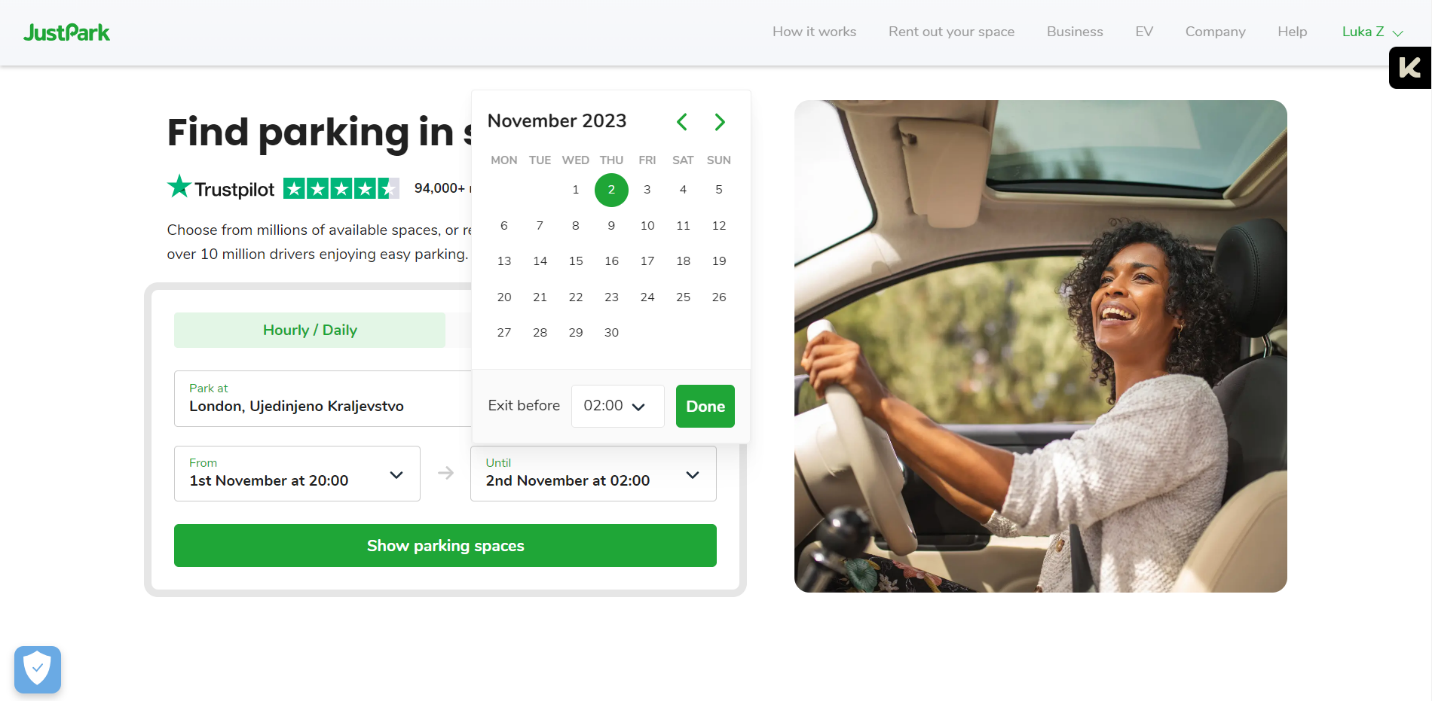
\includegraphics[]{slike/justPark1.png}}
		\caption{Sučelje za odabir termina u JustPark}
		\label{fig:justpark1}
	\end{figure}
	
	\begin{figure}[!ht]
		\centering
		\fbox{\includegraphics[]{slike/justPark2.png}}
		\caption{Dodatna mogućnost ocjene parkinga u JustPark}
		\label{fig:justpark2}
	\end{figure}
	
	\clearpage
	
	\hspace{1cm}{\Large SpotPicker je aplikacija savršena za ljude koji planiraju svoja putovanja ili obaveze po nekoliko dana unaprijed jer će si rezervacijom mjesta ukloniti onaj najgori dio vožnje, a to je lutanje u potrazi za mjestom. Također, pogodno je ljudima koji moraju negdje doći na vrijeme jer ovako mogu značajno bolje procijeniti koliko im je vremena potrebno u vožnji. Isto tako, aplikaciju mogu korisiti i ljudi kojima je parking potreban stalno (npr. jer rade u blizini) jer je moguće da rezervacija bude ponavljajuća iz tjedna u tjedan.\\}
	
	\hspace{1cm}{\Large Naravno, bitno je napomenuti da je ovaj project moguće nadograditi i poboljšati neke njegove stavke. Tako bi korisni dodatak bio mogućnost poništavanja rezervacije uz povrat novca.\\}
	
	\hspace{1cm}{\Large Šta se tiče prilagodbe raznim tržištima, za manje gradove koji imaju puno privatnih kuća u centru, bila bi dobra mogućnost da se vlasnici kuća s dvorištem mogu prijaviti da iznajmljuju svoje dvorište kao parkirno mjesto. Vlasnik dvorišta bi se jednako vodio kao i vlasnik većeg parkirališta, a odabir mjesta bi djelovao na isti način kao i kod velikih parkinga ovisno o veličini dvorišta. Bitno je primijetiti da projekt uključuje rješenje za parkirališta s jednom razinom, tako da bi jedno dodatno moguće proširenje bilo dodati mogućnost odabira kata garaže i tek onda parkirnog mjesta. \\}
	

	
\end{document}
